% vim: set textwidth=78 autoindent:

\subsection{Complemento de Captura de Coordenadas}

% when the revision of a section has been finalized, 
% comment out the following line:
% \updatedisclaimer

El complemento de captura de coordenadas es fácil de usar y provee la 
habilidad para mostrar coordenadas en el canvas del mapa para dos 
sistemas de referencias de coordenadas (CRS).

\begin{figure}[ht]
   \begin{center}
   \caption{Complemento de captura de coordenadas \nixcaption}\label{fig:coordinate_capture_dialog}\smallskip
   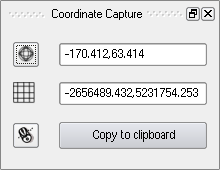
\includegraphics[clip=true, width=9cm]{coordinate_capture_dialog}
\end{center}  
\end{figure}

\begin{enumerate}
  \item Inicie QGIS, seleccione \dropmenuopttwo{mActionOptions}{Propiedades del proyecto} del 
  menú \mainmenuopt{Configuracion} (KDE, Windows) o \mainmenuopt{Archivo} (Gnome, OSX)  
  y clic en la pestaña \tab{Proyección}. Como una alternativa puedes también  
  hacer clic en el ícono \toolbtntwo{mIconProjectionEnabled}{proyector} en la parte 
  inferio derecha de la barra de estado.
  \item Clic en la caja de verificación \checkbox{Activar transformación de SRC al vuelo} y seleccione un 
  sistema de coordenadas proyectadas de tu elección (vea también la sección \ref{label_projections}).
  \item Cargue el complemento de captura de coordenadas en el Administrador de Complementos (vea la sección 
  \ref{sec:load_core_plugin}) y asegúrese que el diálogo está visible yendo a  \mainmenuopt{Ver}
   > \dropmenuopt{Paneles} y asegurándose que \checkbox{Capturar coordenadas} está activo. 
   El diálogo de captura de coordenadas aparece como se muestra en la figura \ref{fig:coordinate_capture_dialog}.
  \item Clic en el ícono \toolbtntwo{geográficas}{Clic para seleccionar el SRC a usar para mostrar coordenadas} 
  y seleccione un SRC diferente del que seleccionó arriba.
  \item Para empezar a capturar coordenadas, clic en \button{Iniciar captura}. Ahora puede hacer clic en cualquier parte 
  del canvas del mapa y el complemento mostrará las coordenadas para los dos sistemas de coordenadas SRC seleccionados.
  \item Para activar el rastreo de coordenadas haga clic en el ícono  \toolbtntwo{rastreo}{rastreo de mouse}.
  \item También puede copiar las coordenadas seleccionadas al portapapeles.
\end{enumerate}

\newpage



